\section{Natural Language Understanding}

The \emph{NLU (natural language understanding)} component of dialogue system produces a semantic representation which is appropriate for the dialogue task. Many speech-based dialogue systems are based on the frame-and-slot semantics \cite{Jurafsky2006}. In this circumstance, the task of NLU is equivalent to filling each slot with the correct value, given the information from the upstream ASR component.

In this section, we begin with presenting some classic approaches for NLU, based on rules, grammar and statistic learning \cite{Miller1996,Pieraccini1994,Ward1994}. Although these methods look simple, they suffice to build several non-trivial dialogue systems that are deployed in real world. The work of Rayner \cite{Rayner2003} aims to proposed a method that can combine both the power of rule-based and data-driven approaches. Several other deep learning techniques proposed recently are also closely related with the NLU component \cite{Hermann2013, Kalchbrenner2013}.

In another line of research, NLU is not restricted to discover merely the value of each slot, but take a more ambitious step to translate the given natural sentence to formal logic or database queries \cite{Grefenstette2014}. These NLU techniques are not yet widely applied in SDS.

Another subject closely related to NLU is called the \emph{dialogue state tracking challenge (DSTC)}. We conclude this section with a paper that address the challenge with LSTM network \cite{Zilka2015} which shows that the NLU component is not always necessary.

\subsection{A Fully Statistical Approach to Natural Language Interfaces \cite{Miller1996}}

This paper presents a natural language interface system which is based entirely on trained statistical models. The system consists of three stages of processing: \emph{parsing}, \emph{semantic interpretation}, and \emph{discourse}. Each of these stages is modeled as a statistical process. The models are fully integrated, resulting in an end-to-end system that maps input utterances into meaningful representation frames.

The focus of this paper is to extract sufficient information from each utterance to give an appropriate response to a user's request. The model structure of this paper is described as follows: Given a string of input words $W$ and a discourse history $H$, the task of statistical language understanding system is to search among the many possible discourse-dependent meanings $M_D$ for the most likely meaning $M_0$:
$$M_0 = \mathop{\arg \max}_{M_D} P(M_D | W, H).$$
Let $T$ denote a semantic parse tree, and $M_S$ denote pre-discourse sentence meaning (the sentence meaning without considering the discourse history) we can introduce intermediate levels into the statistical framework:
$$M_0 = \mathop{\arg \max}_{M_D} \sum_{M_S, T} P(M_D | W, H, M_S, T) P(M_S, T | W, H).$$

The representation can be further simplified with the following three assumptions: 1) Neither the parse tree $T$, nor the pre-discourse meaning $M_S$, depends on the discourse history $H$. 2) The post-discourse meaning $M_D$ does not depend on the words $w$ or the parse structure $T$, once the pre-discourse meaning $M_S$ is determined. 3) The probability of words $W$ does not depend on meaning $M_S$, given that parse $T$ is known. Finally, these assumptions yield the following objective function:
$$M_0 = \mathop{\arg \max}_{M_D} (\max_{M_S, T}(P( M_D | H, M_S) P(M_S, T) P(W | T))).$$
\begin{figure}[h]
  \centering
  % Requires \usepackage{graphicx}
  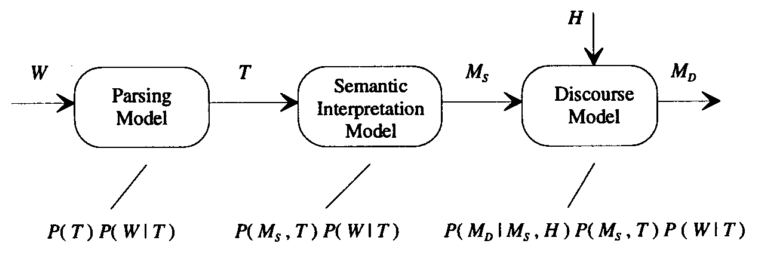
\includegraphics[width=.9\linewidth]{stat_NLI1.png}\\
  \caption{Overview of statistical processing}\label{fig:stat_NLI1}
\end{figure}

This expression corresponds to the computation actually performed by the system which is shown in Figure \ref{fig:stat_NLI1}. The processing proceeds in three stages:
\begin{enumerate}
\item Word string $W$ arrives at the parsing model. The fill space of possible parses $T$ is searched for $n$-best candidates according to the measure $P(T)P(W|T)$. These parses, together with their probability scores, are passed to the semantic interpretation model. The probability $P(T)$ is modeled by state transition probabilities in a recursive transition network, and $P(W|T)$ is modeled by word transition probabilities. Here state transition probabilities have the form $P(state_n | state_{n-1}, state_{up})$, and word transition probabilities have the form $P(word_n | word_{n-1}, tag)$.
\item The constrained space of candidate parses $T$, combined with the full space of possible pre-discourse meanings $M_S$, is searched for $n$-best candidates according to the measure $P(M_s, T)P(W|T)$. These pre-discourse meanings, together with their associated probability scores, are passed to the discourse model. Both pre-discourse and post-discourse meanings in the current system are represented using a simple frame representation (cf. Figure \ref{fig:stat_NLI2}). The problem in this stage is to compute the prior probability of meaning $M_S$ and parse $T$ occurring together. The method of this paper is to embed the instructions for constructing $M_S$ directly into parse $T$. So the probability $P(M_S, T)$ is then simply the prior probability of producing the augmented tree structure.
    \begin{figure}[h]
      \centering
      % Requires \usepackage{graphicx}
      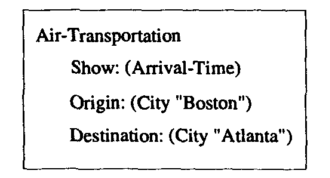
\includegraphics[width=.4\linewidth]{stat_NLI2.png}\\
      \caption{A sample semantic frame}\label{fig:stat_NLI2}
    \end{figure}
\item The constrained space of candidate pre-discourse meanings $M_S$, combined with the full space of possible post-discourse meanings $M_D$, is searched for the single candidate that maximizes $P(M_D | H, M_S)P(M_S, T)P(W|T)$, conditioned on the current history $H$. The discourse history is then updated and the post-discourse meaning is returned. The discourse history $H$ simply consists of the list of all post-discourse frame representations for all previous utterances in the current session. Let $M_P$ denote the last frame in the list. The statistical discourse model maps a 23 element input vector onto a 23 element output vectors. Here $X$ represents the combination of $M_P$ and $M_S$, while $Y$ represents the post-discourse meaning $M_D$. Finally, the probability $P(Y | X)$ is determined by a statistical decision tree model.
\end{enumerate}

In the experimental study, the paper trained and evaluated the system on a common corpus of utterances collected from naive users in the \emph{ATIS} domain. The combined system produced an error rate of 21.6\%, and work on the system was still ongoing. 
\subsection{A Learning Approach to Natural Language Understanding \cite{Pieraccini1994}}

This paper proposes a learning paradigm for the problem of understanding spoken language. The basis of the work is in a formalization of the understanding problem as a communication problem. The resulting understanding algorithm consists in a Viterbi maximization procedure analogous to that commonly used for recognizing speech.

The first step of this paper is to formalize the NLU problem as a \emph{communication problem}. Two assumptions are made in this step: 1) the meaning of a sentence can be expressed by a sequence of basic units $\mM = \mu_1, ..., \mu_{N_M}$, and there is a sequential correspondence between $\mu_j$ and a subsequence of the acoustic observation $A = a_1, ..., a_{N_a}$; 2); 2) the second assumption is to think of the acoustic representation as a version of the original sequence of meaning units corrupted by a noisy channel. Thus for a given acoustic observation $A$, the problem of understanding a sentence can be expressed as finding $\mathop{\max\arg}_\mM P(\mM | A)$.

A simple choice is to define a unit of meaning as a keyword/value pair $m_j = (k_j, v_j)$, where $k_j$ is a conceptual category (e.g. origin, meal) and $v_j$ is the value in the actual sentence (e.g. Boston, breakfast). In what follows we use $W = w_1, ..., w_{N_W}$ to denote the sequence of words, and use $C = c_1, ..., c_{N_W}$ to denote the sequence of concept labels.

Using the Bayesian rule, the formula can be expressed as:
$$\mathop{\max\arg}_{W,C} P(A | W, C) P(W | C) P(C).$$
It is further assumed that:
$$P(w_i | w_{i-1}, ..., w_1, C) = P(w_i | w_{i-1}, ..., w_{i-n+1}, c_i),$$
$$P(c_i | c_{i-1}, ..., c_1) =  P(c_i | c_{i-1}, ..., c_{i-m}).$$
When $n=m=1$, this is equivalent to a first order \emph{hidden Markov model (HMM)}.

\begin{figure}[h]
  \centering
  % Requires \usepackage{graphicx}
  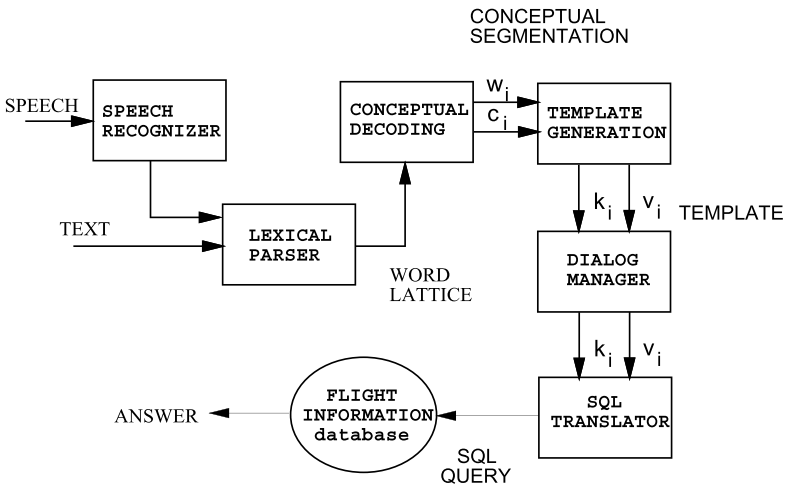
\includegraphics[width=.8\linewidth]{P94-NLU_diag.png}\\
  \caption{Block diagram of the understanding system.}\label{fig:P94-NLU_diag}
\end{figure}

The paper then presents how to implement this idea and apply it to the \emph{ATIS (Air Travel Information System)} corpus. A block diagram of the speech understanding system is presented in Figure \ref{fig:P94-NLU_diag}. Next we will see each of the components in further detail.

In the \emph{conceptual decoding} module, the paper proposes to impose a certain structure to the HMM. It is observed that in a typical sentence there are phases that generally represent the question, a subject and finally a restriction. So the HMM follows this structure to alleviates the problems of the locality of the model and that of concept embedding.

The \emph{lexical parser} dues with different issues related with spoken language, such as the representation of numbers and acronyms. The lexical parser also deletes articles (i.e. THE and A), since they play no role in the conceptual decoding process.

The paper uses the most natural way of \emph{interfacing} the conceptual decoder with a speech recognizer, by directly implementing the maximization of the probability described above. In order to manage the model size, it uses only those words and bigrams that were observed in the training data.

The goal of the \emph{template generator} module is to analyze the conceptual segmentation, and generate the final representation of the meanings. Finally values are assigned to the decoded concepts according to the result of a pattern matching procedure. However, the design of pattern matching tables still requires manual efforts.

The \emph{dialog manager} implements the function of recording the dialog history, and generates proper responses. The simple strategy used in the paper is to keep a current context template, with all the information that has been used. If a concept is mentioned in a new sentence but with a different value, all concepts in the context template at a lower hierarchical level are deleted.

In the experimental study, the proposed system was evaluated on a set of 687 sentences called February 92 test set. The results on the test set from text input account for 68\% of correct answers, 18\% wrong answers and 14\% rejects. When the system was coupled with a speech recognizer through the best first hypothesis, the performance dropped to 52\% of correct answers, 26\% wrong answers and 22\% rejects.

\subsection{Recent Improvements in the CMU Spoken Language Understanding System \cite{Ward1994}}

A spoken language system needs to recognize and understand spontaneous speech, which often contains disfluencies and ungrammatical construction. The goal of this paper is to develop a NLU system that can respond appropriately to input, even though coverage is not complete.

The CMU NLU system is called \emph{Phoenix}, which has a loose coupling between the speech recognizer. The recognizer uses stochastic language models to produce a single word string hypothesis. This hypothesis is then passed to a parsing module which uses semantic grammars to produce a semantic representation for the input utterance.

The basic idea of this paper is to use a flexible frame-based parser, which parses as much of the input as possible. The Phoenix system uses \emph{Recursive Transition Networks} to encode semantic grammars. The grammars specify word patterns which correspond to semantic tokens understood by the system. A subset of tokens are considered as top-level tokens, which means they can be recognized independently of surrounding context. Nets call other nets to produces a semantic parse tree. The top-level tokens appear as slots in the frame structures. There is not one large sentential-level grammar, but separate grammars for each slot (there are approximately 70 of these in the ATIS system). The parser is flexible at the slot level in that it allows slots to be filled independent of order.

The parser operates by matching the word patterns for slots against the input text. A set of possible interpretations are pursued simultaneously. The system is implemented as a top-down Recursive Transition Network chart parser for slots. As slot fillers are recognized, they are added to frames to which they apply. At the end of an utterance the parser picks the best scoring frame as the result. The output of the parser is the frame name and the parse trees for its filled slots.

The semantic grammar used for parsing in the ATIS task is developed by processing transcripts of subjects performing scenarios. The data consists of around 20,000 utterances, and a subset of this data (around 10,000 utterances) has been annotated. However, it has a problem with the grammar coverage if it misses one of the content words in the utterance. The paper tries to solve this problem by generalizing the grammar to parse strings that are syntactically similar to the utterances in the training data.

The paper also found it helpful to pursue alternate interpretations, which are not the best according to the heuristics used by the parser. This is achieved by generating a beam of interpretations. The parser still produces the single best interpretation, but keeps track of a number of others. Whenever the backend notices a problem, it asks the parser for another interpretation.

In the experimental study, it is reported that the error rates of the speech recognizer, NLU component and the overall system are 4.4\%, 9.3\% and 13.2\% respectively.

\subsection{Transparent Combination of Rule-based and Data-driven Approaches in a Speech Understanding Architecture \cite{Rayner2003}}

This paper describes a domain-independent semantic interpretation architecture suitable for spoken dialogue systems, which uses a decision-list method to effect a transparent combination of rule-based and data-driven approaches.

The goal of the paper is to propose an architecture which combines rule-based and data-driven methods as transparently as possible. This will allow the system to shift smoothly from an initial version which is entirely rule-based, to a final version which is largely data-driven.

In this paper, \emph{semantic interpretation} is viewed as a statistical \emph{classification} task. There is a set of semantic atoms, each representing a primitive domain concept, and a semantic representation is defined to be a non-empty set of semantic atoms. For example, the semantic representation of the utterance ``show me the sample syringe'' is $\{show, sample\_syringe\}$. As well as specifying the permitted semantic atoms themselves, it also defines a target model which for each atom specifies the other atoms with which it may legitimately combine. For example, $minutes$ may only combine with $correction$, $set\_alarm$ or a number.

Training data consists of a set of utterances, in either text or speech form, each tagged with its intended semantic representation. The paper defines a set of feature extraction rules, each of which associates an utterance with zero or more features. Statistics are then compiled to estimate the probability $p(a | f)$ of each semantic atom $a$ given each separate feature $f$.

In the decoding process, the system is given an utterance $u$, to which the system assigns a representation $R(u)$ consisting of a set of semantic atoms, together with a target model. The decoding process  proceeds as follows:
\begin{enumerate}
\item Initialise $R(u)$ to the empty set.
\item Use the feature extraction rules and the compiled statistics to find the set of triples $\langle f, a, p \rangle$ where $f$ is a feature associated with $u$, $a$ is a semantic atom, and $p$ is the probability $p(a | f)$.
\item Order the set of triples by the value of $p$, with the largest probabilities first.
\item Remove the highest-ranked triple $\langle f,a,p \rangle$ from $T$. Add $a$ to $R(u)$ if the probability $p$ is greater than some threshold and $a$ is consistent with $R(u)$.
\end{enumerate}

The paper describes an open-source toll called $ALTERF$, which implements the abstract procedure introduced above. It shows how the $ALTERF$ system processes the training data, and decodes the given utterance in running time with further details.

In the experimental study, the paper shows that when all the training data is used, the combined system outperforms the rule-based system by 22.2\% to 27.3\%, and outperforms the N-gram system by 22.2\% to 25.6\%. It shows that the proposed method can get a significant improvement on rules-based technique by adding a trainable component. 
\subsection{Multilingual Distributed Representations without Word Alignment \cite{Hermann2013}}

This paper proposes a method for learning distributed representations in a multiligual setup. The model learns to assign similar embeddings to aligned sentences and dissimilar ones to sentences which are not aligned. It shows that the representations are semantically informative and applies them to a cross-lingual document classification task.

The basic idea is that, given enough parallel data, a shared representation would be forced to capture the common elements between sentences from different languages. What two parallel sentences have in common, of course, is the semantics of those two sentences. Using such parallel data, it proposes a novel method for learning vector representations at the word level and beyond.

The first step is to define a bilingual error function as follows: given a \emph{compositional sentence model (CVM)} $\mM_A$, which maps a sentence to a vector, it trains a second CVM $\mM_B$ using a parallel corpus $\mC_{A,B}$. For each pair of parallel sentences $(a,b) \in \mC_{A,B}$, it attempts to minimize
$$E_{dist}(a,b) = ||a_{root} - b_{root}||^2,$$
where $a_{root}$ ($b_{root}$) is the vector representing sentence $a$ ($b$).

The CVM used in this paper is a simple additive composition function:
$$a_{root}= \sum_{i=0}^{|a|} a_i.$$
Due to the use of parallel data, we know that $a$ and $b$ are semantically equivalent. Hence the goal is to jointly train both models $\mM_A$ and $\mM_B$, so that
$$E_{bi}(\mC_{A,B}) = \sum_{(a,b) \in \mC_{A,B}} E_{dist}(a,b)$$
is minimized.

However, the models could learn to reduce all embeddings and composition weights to zeros and thereby minimize the objective function. This problem is addressed by penalizing small distances between non-parallel sentence pairs. For every pair of parallel sentences $(a,b)$ it samples a number of additional sentences $n \in \mC_B$, which are not exact translation of $a$:
$$E_{noise}(a, b, n) = [1 + E_{dist}(a,b) - E_{dist}(a,n)]_{+},$$
where $[x]_{+} = \max(x,0)$ denotes the standard hinge loss. Thus, the final objective function is defined to be:
$$J(\theta_{bi}) = \sum_{(a,b) \in \mC_{A,B}} (\sum_{i=1}^k E_{noise}(a,b,n_i)) + \frac{\lambda}{2} || \theta_{bi} ||^2.$$

\begin{figure}[h]
  \centering
  % Requires \usepackage{graphicx}
  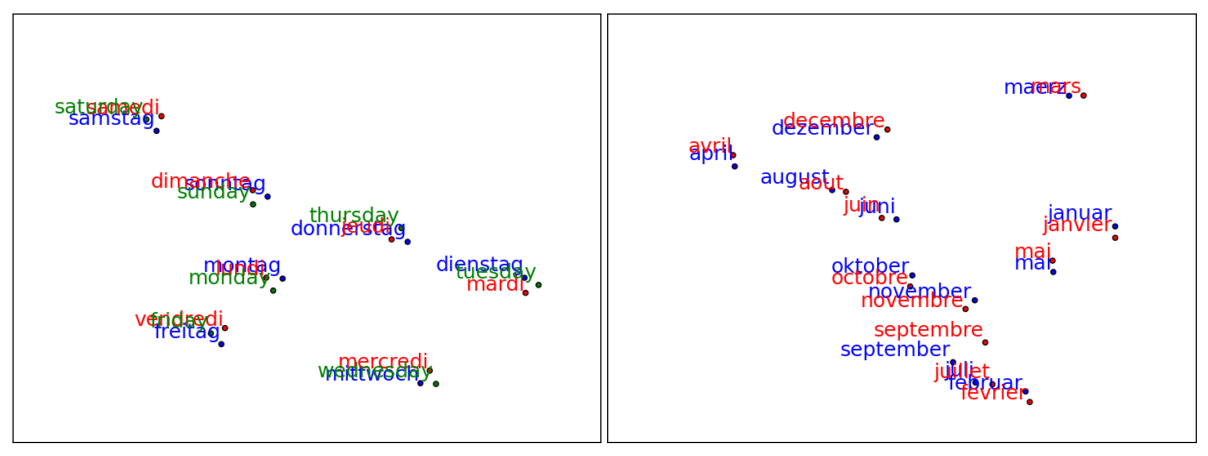
\includegraphics[width=\linewidth]{Hermann13-BiCVM.png}\\
  \caption{The left scatter plot shows t-SNE projections for a weekdays in three language. The right plots shows months using only the German and French words.}\label{fig:Hermann13-BiCVM}
\end{figure}

In the experimental study, the paper evaluates the proposed model in to experiments: the \emph{BiCVM} model was trained on 500k sentence pairs of a English-German parallel corpus. The \emph{BiCVM+} used this dataset in combination with anther 500k parallel sentences form the English-French section. The motivation behind BiCVM+ is to investigate whether it can learn better embeddings by introducing additional data in a different language. The models are evaluated on the \emph{cross-lingual document classification (CLDC)} task. It is shown that both models outperform all prior work on this task. Further, BiCVM+ outperforms BiCVM, indicating the usefulness of adding training data from a separate pair. Figure \ref{fig:Hermann13-BiCVM} shows the t-SNE projections for a number of English, French and German words.

\subsection{Recurrent Convolutional Neural Networks for Discourse Compositionality \cite{Kalchbrenner2013}}

This paper introduces both a sentence model and a discourse model corresponding to the two levels of compositionality: cords combine to form the meaning of sentences, and sentences combine to form the meaning of dialogues. The sentence model adopts convolution as the central operation, and is based on a novel \emph{hierarchical convolutional neural network (HCNN)}. The discourse model extends the sentence model, and is based on a \emph{recurrent neural network (RNN)}.

The basic kernel operation used in HCNN is described as follows. Given a sentence $s$ and its paired matrix $\mathbf{M}^s$, let $\mathbf{m}$ be a feature that is a row in $\mathbf{M}^s$. Let $w_1, ..., w_k$ be a sequence of $k$ weights. The local weighted addition over the first $k$ values is:
$$y = w_1 \mathbf{m}_1 + ... + w_k \mathbf{m}_k.$$
Then a kernel simply defines the value of $k$, and the one-dimensional convolution applies local weighted addition to each subsequence of values of $\mathbf{m}$. The one-dimensional convolution ($\mathbf{k} * \mathbf{m}$) is defined as:
$$(\mathbf{k} * \mathbf{m})_i = \sum_{j=1}^k \mathbf{k}_j \cdot \mathbf{m}_{k+i-j}.$$

To define the hierarchical architecture of the model, the paper next defines a sequence of kernel sizes and associated weights. Let $l$ be the number of words in the sentence $s$. The sequence of kernel sizes is defined as
$$k_1^l = 2, k_{i+1}^l = k_i^l + 1, k_t^l = l - \sum_{j=1}^{t-1}(k_j^l - 1).$$
That is, kernel sizes increase by one until the resulting convolved vector is smaller or equal to the last kernel size (cf. Figure \ref{fig:Kal13-hier}).

\begin{figure}[h]
  \centering
  % Requires \usepackage{graphicx}
  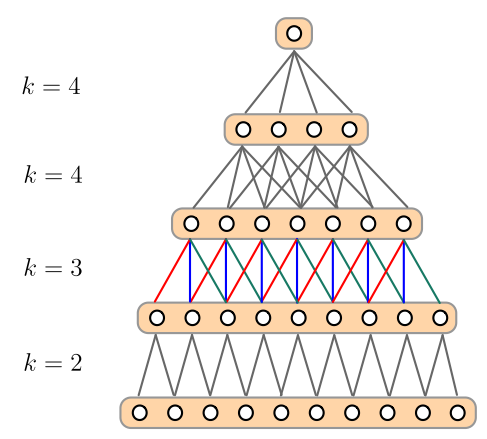
\includegraphics[width=.6\linewidth]{Kal13-hier_HCNN.png}\\
  \caption{A hierarchical convolutional neural network for sentential compositionality.}\label{fig:Kal13-hier}
\end{figure}

The composition operation in HCNN is formally defined as follows. For each feature $f$, let $\mathbf{K}_i^f$ be a sequence of $t$ kernels, where the size of the kernel $|\mathbf{K}_i^f| = k_i^l$. The hierarchy of matrices and corresponding features are defined as:
\begin{align*}
\mathbf{M}_{f,:}^1 &= \mathbf{M}_{f,:}^s,\\
\mathbf{M}_{f.:}^{i+1} &= \sigma(\mathbf{K}_i^f * \mathbf{M}_{f,:}^i + b_f^i).
\end{align*}

The discourse model adapts a RNN architecture in order to capture central properties of discourse. The proposed method aims to capture at least two of the most prominent properties: the sequentiality of the utterances, and the interactions between the speakers.

The RNN architecture takes inputs from a HCNN conditioned on the respective speakers. Let $s_1, ..., s_T$ be a sequence of sentences, each in turn being a sequence of words $s_i = y_1 ... y_l^i$. Let $x_1, ..., x_T$ be a sequence of labels, and $a_1, ..., a_T$ be a sequence of speaker. The RNN computes probability distribution by iterating the following equations:
\begin{align*}
\mathbf{h}_i &= \sigma(\mathbf{I} x_{i-1} + \mathbf{H}^{i-1}\mathbf{h}_{i-1} + \mathbf{Ss}_i + b_h)\\
         p_i &= softmax(\mathbf{O}^i \mathbf{h}_i + b_o)
\end{align*}

\begin{figure}[h]
  \centering
  % Requires \usepackage{graphicx}
  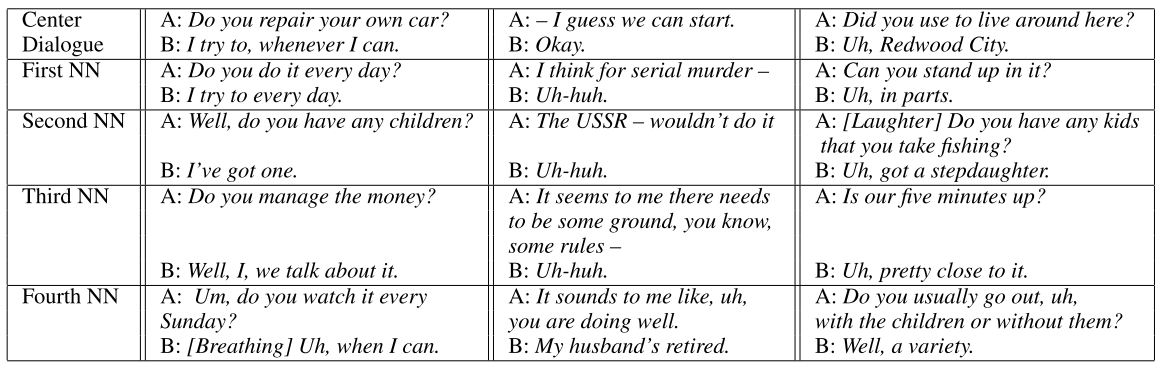
\includegraphics[width=\linewidth]{Kal13-NN.png}\\
  \caption{Short dialogues and nearest neighbours.}\label{fig:Kal13-NN}
\end{figure}

In the experimental study, the paper evaluates the proposed model with the prediction of dialogue acts within the \emph{Switchboard Dialogue Act corpus}. The RCNN model achieves prediction accuracy of 73.9\%, while the best previous result was 71.0\%. Figure \ref{fig:Kal13-NN} shows three randomly chosen dialogues, and the four nearest neighbours of each.

\subsection{A Deep Architecture for Semantic Parsing \cite{Grefenstette2014}}

This paper presents a novel deep learning architecture which provides a semantic parsing system through the union of two neural models of language semantics. It allows for the generation of ontology-specific queries from natural language statements and questions without the need for parsing, which makes it especially suitable to grammatically malformed or syntactically atypical text such as tweets.

The goal of \emph{semantic parsing} is to map natural language sentences to formal representations of their underlying meaning. Within the context of question answering - the focus of this paper - semantic parsing typically aims to map natural language to database queries that would answer a given question.

The model proposed in the paper borrows from two approaches in the deep learning literature: the \emph{Bilingual Compositional Sentence Model (BiCVM)} and \emph{Conditional Neural Language Model (CNLM)}.

\begin{figure}[h]
  \centering
  % Requires \usepackage{graphicx}
  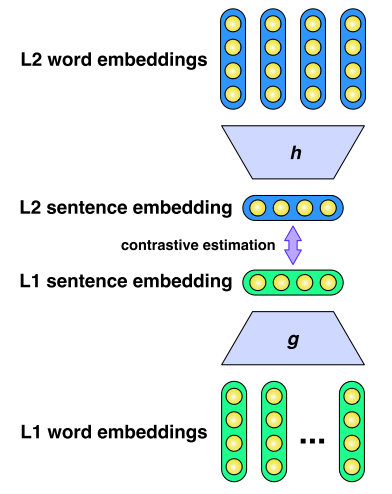
\includegraphics[width=.5\linewidth]{G2014-BiCVM.png}\\
  \caption{Diagrammatic representation of a BiCVM.}\label{fig:BiCVM}
\end{figure}

The BiCVM model shown in Figure \ref{fig:BiCVM} assumes vector composition functions $g$ and $h$, which map an ordered set of word embeddings onto a single vector. For semantically equivalent sentences $a, b$ across different languages (for example English and Chinese), the model aims to minimise the distance between these composed representations:
$$E_{bi}(a,b) = ||g(a) - h(b)||^2.$$
This error is combined with a noise-contrastive hinge loss, where $n$ is a randomly sampled sentence dissimilar to the parallel pair $\{a,b\}$, and $m$ denotes some margin:
$$E_{hl}(a,b,n) = max(0, m + E_{bi}(a,b) - E_{bi}(a,bn)).$$

A \emph{log-bilinear language model} is a neural network modelling a probability distribution over the next word in a sequence given the previous $n-1$, i.e. $p(w_n | w_{1:n-1})$. Let $C_i$ be the context transform matrix which modifies the representation of the $i$th word in the word history. Let $b_{w_i}$ be a scalar bias associated with a word $w_i$, and $b_R$ be a bias vector associated with the model. A log-bilinear model expressed the probability of $w_n$ as a function of the energy of the network:
$$E(w_n ; w_{1:n-1}) = -(\sum^{n-1}_{i=1}R_{w_i}^T C_i) R_{w_n} - b_R^T R_{w_n} - b_{w_n}.$$
To reframe a log-bilinear language model as a CNLM, the simplest way is to do this additively, which allows us to treat the contribution of the conditional variable $\beta$ as an extra word in the history.

The models described above can be combined to form a model capable of jointly learning a shared latent representation for question/query pairs using a BiCVM, and using this latent representation to learn a conditional log-bilinear CNLM.

\begin{figure}[h]
  \centering
  % Requires \usepackage{graphicx}
  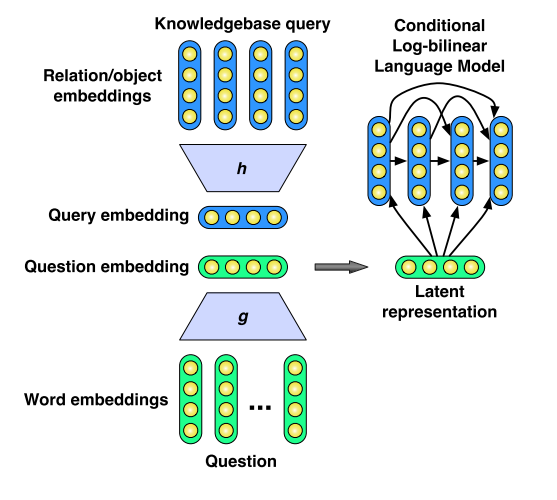
\includegraphics[width=.6\linewidth]{G2014-combined.png}\\
  \caption{Diagrammatic representation of the combined model.}\label{fig:G2014-combined}
\end{figure}

Figure \ref{fig:G2014-combined} shows the combined model. For the natural language side of the model, the composition function $g$ can be a simple additive model. Function $h$, which maps the knowledge base queries into the shared space could use a convolution neural network. Using function $g$ and the original training data, the training data for the second stage is created by obtaining the latent representation for the questions of the original dataset. Once trained, the models can be fully joined to produce a generative neural network.

Finally, the paper suggests that the proposed model can be trained in a two-stage process, and discusses the experimental requirements. However, there is no implementation when the paper is published. So it is left as future work whether the proposed training method can yield fruitful results in practice.

\subsection{Incremental LSTM-based Dialog State Tracker \cite{Zilka2015}}

A dialog state tracker estimates the user's goal throughout the dialog by analyzing the \emph{automatic speech recognition (ASR)} outputs for the user's utterance. This paper presents an incremental dialog state tracker based on LSTM networks. It directly uses ASR hypothesis to track the state.

Because of uncertainty in the user input, statistical dialog systems maintain a distribution over all possible states, called the belief state. In this paper, a dialog state at time $t$ is defined as a vector $s_t \in C_1 \times ... \times C_k$ of $k$ dialog state components (sometimes also called slots). Each component $c_i \in C_i = \{ v_1, ..., v_{n_i} \}$ takes one of $n_i$ values. The goal of the dialog state tracker is to give the probability distribution over one of the independent components $p(c_i | w_1, ..., w_t)$.

\begin{figure}[h]
  \centering
  % Requires \usepackage{graphicx}
  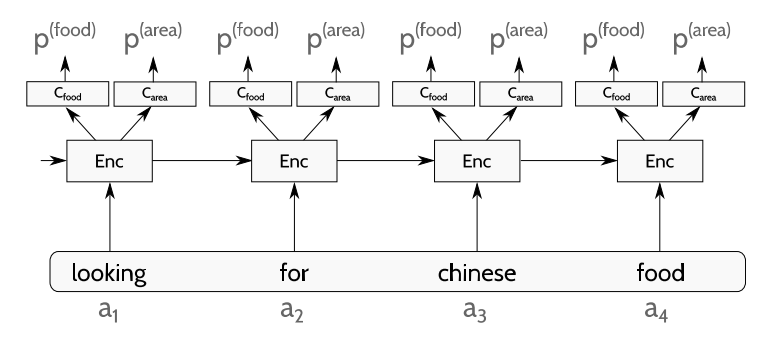
\includegraphics[width=.7\linewidth]{11_28_dstc_ilstm.png}\\
  \caption{A demonstration of the proposed model}\label{fig:dstc_ilstm}
\end{figure}

The main idea of this paper is to use LSTM to encode the information from the input word sequence into a fixed-length vector representation. Given this representation, a classifier returns a probability distribution over the value of the dialog state. An example of the model applied to a particular input sentence is at Figure \ref{fig:dstc_ilstm}.

Formally, the input neural network maps the word $a$ and its ASR confidence score $r$ to a joint representation $u$: $u = NN(a, r)$. The representation $u$ is used by the LSTM encoder along with the previous hidden state $q_{t-1} = (c_{t-1}, h_{t-1}$ to create a new hidden state $q_t$: $q_t = Enc(u, q_{t-1})$. The classifier, represented by a single softmax layer, then maps the hidden state to a probability distribution over all possible values: $p_t = C(h_t)$.

The training criterion is a cross-entropy loss for a dialog example, which is annotated by true labels at some points in time:
$$l(\theta) = - \sum_{t \in Y} \log LecTrack(a_1, r_1, ..., a_n, r_n)_{y_t}^t,$$
where $y_i$ denotes a label for the dialog state at time $i$, and $Y$ is a set of times where the label $y_i$ exists.

In the experimental study, the paper shows that the propose model yields performance to the state-of-the-art system. For example in the requested component, the proposed method achieves 0.98 accuracy and 0.04 L2 score, which is identical to the result of the previous best system. 
